% id: 0315
% book: RPM 기하 · 03 공간도형
% section: 유형 11 정사영의 넓이를 이용하여 각의 크기 구하기
% figure: crop:fig-0315.png
% answer: $\dfrac{1}{8}$
% answer_source: 답지(쪽 렌더)
% variant_level: 0 (원본 전사)
% 이 파일은 build.mjs 가 items.json 에서 만든다. 고칠 때는 items.json 을 고친다.
\smash{\raisebox{1.5mm}{\dmkichul{RPM 기하 0315번 · 51쪽}}}
\noindent\begin{minipage}[t]{0.58\linewidth}\vspace{0pt}\raggedright 오른쪽 그림과 같이 한 변의 길이가 $1$인 정사각형을 밑면으로 하고 $\seg{AB}=\seg{AC}=\seg{AD}=\seg{AE}$인 사각뿔에서 삼각형~$\pt{ABC}$의 넓이는 $2$이다. 평면~$\pt{ABC}$와 평면~$\pt{BCDE}$가 이루는 각의 크기를 $\theta$라 할 때, $\cos\theta$의 값을 구하시오.\end{minipage}\hfill\begin{minipage}[t]{0.4\linewidth}\vspace{0pt}\centering \setlength{\dmfigw}{94.9pt}\ifdim\dmfigw>\linewidth\setlength{\dmfigw}{\linewidth}\fi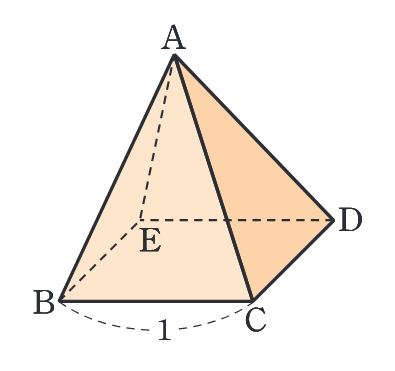
\includegraphics[width=\dmfigw]{figures/fig-0315.png}\end{minipage}\par
